\subsection{Study design and analysis hierarchy}
We compare training targets while matching architecture, initialization, image order, augmentation and optimization within each backbone and seed. The original four adaptive phases contain 24 runs and 48 retained validation-selected or epoch-12 states (Table~\ref{tab:phases}). Initial Hard/Soft results informed the Uniform/Tie-hard follow-up, followed by Tie-Uniform and ResNet-18 checks. Each phase was specified before its own training and calibration/test outcomes, but earlier PrivateTest results were known. These phases therefore provide adaptive within-source evidence.

The 80\% coverage endpoint was fixed in the original Hard/Soft protocol. The later Soft-minus-Uniform protocol inherited this reporting point and designated that contrast primary before its new outcomes. It was not chosen to maximize the observed follow-up effect and is not asserted to be an optimal operating point; other coverages are sensitivities. Distribution-distance summaries, confidence-score analyses and external diagnostics have the secondary or exploratory roles stated below. Follow-up target and vocabulary tests were specified after reviewing these earlier results and frozen before their own outcomes; they do not create an untouched confirmatory test.

The RAVDESS plan was frozen locally before external model outcomes, after internal findings and annotation summaries were known. A retained pre-analysis amendment corrected swapped disgust/surprise response indices against source descriptors and accuracy records before computing external metrics. Protocols, input hashes, phase freezes and the amendment accompany the release. The design does not constitute external preregistration.
\begin{table}[!htbp]
\caption{Adaptive experimental phases on the same source; every phase uses seeds 17, 42, 89 and selected/fixed-epoch evaluation}\label{tab:phases}
\centering\begin{tabular}{llrl}\toprule
Phase & Target conditions & Runs & Prior outcomes known\\\midrule
1 & Hard, Soft & 6 & Historical results\\
2 & Uniform, Tie-hard & 6 & Phase 1\\
3 & Tie-Uniform & 3 & Phases 1 and 2\\
4 & ResNet soft controls & 9 & Phases 1--3\\
\bottomrule\end{tabular}\par
Phase 4 compares Soft, Uniform and Tie-Uniform. All phases retain the same roles and matched within-backbone, within-seed optimization. These are not independent-source replications.
\end{table}


\subsection{Data provenance and isolated roles}
FER2013 has 28,709 Training, 3,589 PublicTest and 3,589 PrivateTest rows. A Kaggle-mirror image CSV was joined to official FER+ counts by original row and partition using the official conversion indexing. Acquired-source hashes establish consistency with that archive, not independent photograph authenticity or rights. Images are not redistributed.

Exact pixel hashes define the roles in Table~\ref{tab:roles}. Training is unchanged. Removing 280 PublicTest rows matching Training leaves pixel clusters assigned to selection or calibration by a fixed label-independent hash. Removing 314 PrivateTest rows matching Training or any PublicTest row leaves 3,275 primary test images. Exact pixels are disjoint across roles; person and near-duplicate separation remain unverified. Full PrivateTest outputs remain available for audit.
\begin{table}[!htbp]
\caption{Operational roles after exact-pixel isolation. Counts are images, not people}\label{tab:roles}
\centering\begin{tabular}{lrl}\toprule
Source and role & Images & Use\\\midrule
Training & 28,709 & Optimization\\
PublicTest: selection & 1,667 & Checkpoint choice\\
PublicTest: calibration & 1,642 & Threshold choice\\
PrivateTest: primary & 3,275 & Main evaluation\\
PrivateTest: full & 3,589 & Prediction archive\\
\bottomrule\end{tabular}\end{table}


\subsection{Training targets}
Let $q_{ic}$ be the fraction of image $i$'s annotations assigned to category $c$, normalized over the ten FER+ response categories. The original supported outputs are angry, disgust, fear, happy, neutral, sad and surprise; contempt, unknown and not-a-face are retained in scoring. Define $w_i=\sum_{c=1}^{7}q_{ic}$ and $r_{ic}=q_{ic}/w_i$ for $w_i>0$. For model probabilities $p_{ic}$,
\begin{align}
\ell_i^{\mathrm{Hard}}&=-w_i\log p_{ih_i},\quad h_i=\arg\max_{c\leq7}r_{ic},\\
\ell_i^{\mathrm{Soft}}&=-w_i\sum_{c=1}^{7}r_{ic}\log p_{ic}
=-\sum_{c=1}^{7}q_{ic}\log p_{ic}.
\end{align}
Loss averages over batch size, not summed weights. All targets use the same images and $w_i$; 152 zero-supported-mass Training rows have zero supervised loss. Hard resolves the 1,360 positive-mass tied maxima by fixed class order.

Uniform preserves $m_i=\max_c r_{ic}$ at the first maximum $h_i$, assigning $(1-m_i)/6$ elsewhere. Tie-hard assigns $1/|T_i|$ to every tied maximum $T_i=\{c:r_{ic}=m_i\}$ and zero elsewhere: the expected loss from uniform tie resolution. Tie-Uniform preserves every tied maximum. For $k_i=|T_i|<7$,
\begin{equation}
t_{ic}^{\mathrm{TU}}=\begin{cases}m_i,&c\in T_i,\\(1-k_i m_i)/(7-k_i),&c\notin T_i.\end{cases}
\end{equation}
When $k_i=7$, all entries equal $1/7$. Each control minimizes $-w_i\sum_c t_{ic}\log p_{ic}$. Figure~\ref{fig:targets} illustrates the target interventions and their measured class-marginal differences. Uniform and Tie-Uniform change entropy and aggregate class proportions; they do not isolate minority-category identity alone. The probability-preserving follow-up is defined in Sect.~\ref{sec:followup}.

\begin{figure}[!htbp]
\centering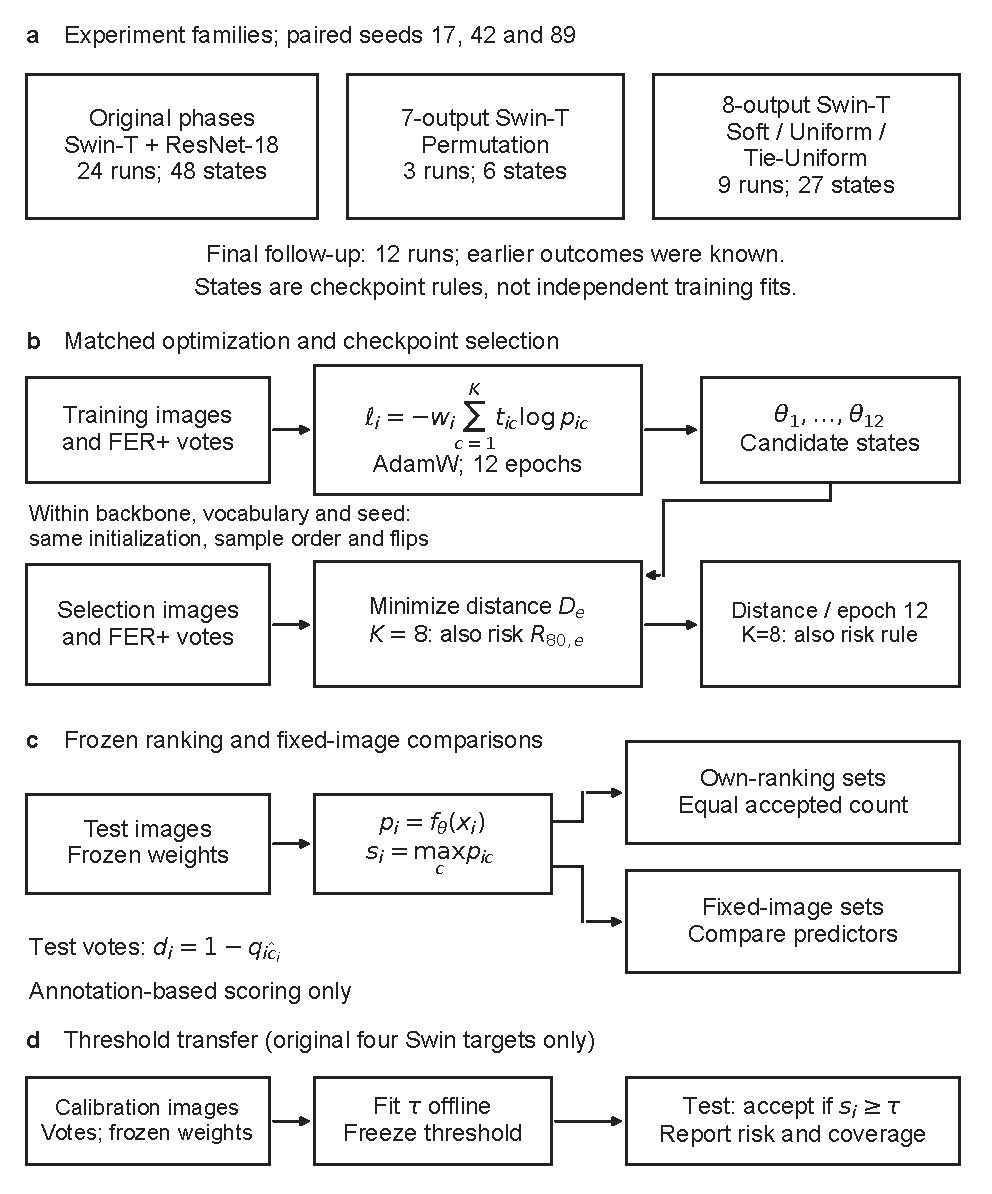
\includegraphics[width=\linewidth]{final_revision_2026_10_20/source/figures/StudyDesign.pdf}
\caption{Study design and adaptive follow-up. (a) Original experiments and the final twelve-run plan, frozen before its own outcomes after earlier findings were known. State counts identify checkpoint rules, not independent fits. (b) Matched training and selection: $D_e$ is selection-set complete-vocabulary squared distance; eight-output models additionally retain a separate state minimizing selection-set 80\% MSP disagreement $R_{80,e}$. Epoch 12 is retained independently. (c) Own-ranking fixes accepted counts; cross-evaluation fixes images. (d) Only the original Hard, Tie-hard, Uniform and Soft policy comparison fits calibration thresholds}\label{fig:design}
\end{figure}
\begin{figure}[!htbp]
\centering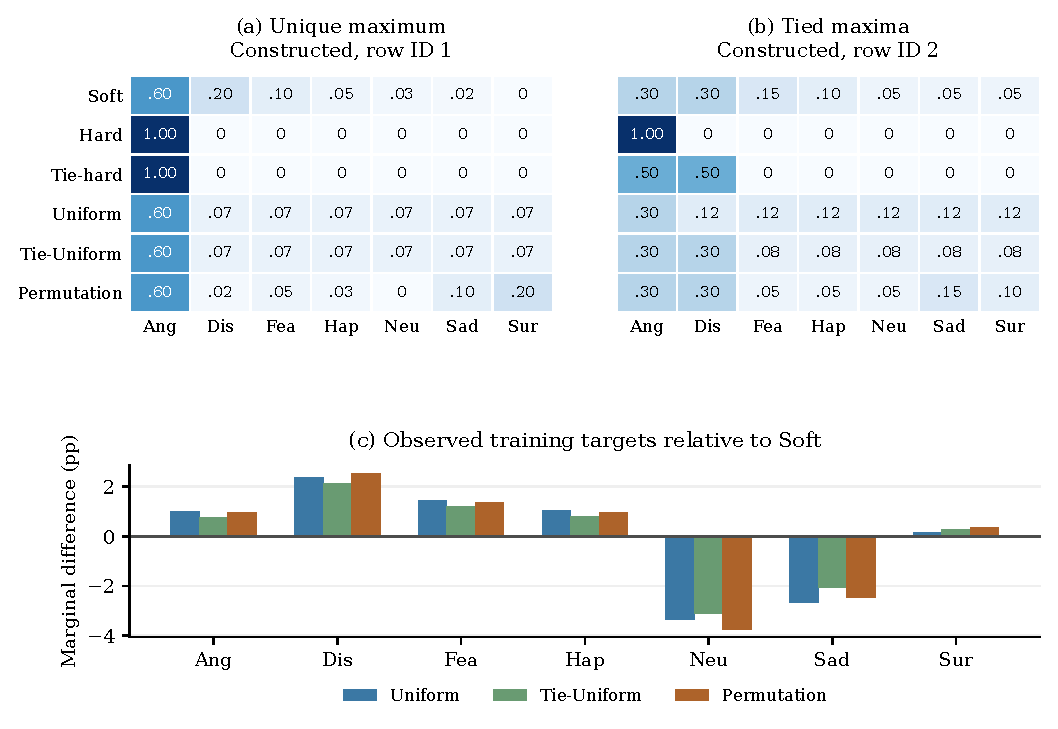
\includegraphics[width=\linewidth]{final_revision_2026_10_20/source/figures/TargetIntervention.pdf}
\caption{Training-target interventions. (a,b) Constructed seven-class examples, rounded to two decimals; nominal row IDs 1 and 2 fix the deterministic permutation and are not sampled images. Permutation preserves every maximum position and the probability multiset. (c) Actual Training targets: weighted class marginals $\sum_iw_it_{ic}/\sum_iw_i$ relative to Soft, in percentage points. Zero-mass rows contribute zero weight. Ang, Dis, Fea, Hap, Neu, Sad and Sur denote angry, disgust, fear, happy, neutral, sad and surprise. Equal per-image entropy need not preserve aggregate class proportions}\label{fig:targets}
\end{figure}

\subsection{Models, preprocessing and optimization}
Swin-T uses torchvision ImageNet-1K V1 initialization \cite{liu2021swin,deng2009imagenet,paszke2019pytorch}. One post-pooling channel gate transforms its 768-vector:
\begin{equation}
\tilde z=z\odot\sigma\!\left(W_2\operatorname{ReLU}(W_1z)\right),\quad
W_1\in\mathbb{R}^{48\times768},\ W_2\in\mathbb{R}^{768\times48}.
\end{equation}
The bias-free gate adds 73,728 parameters; a biased linear classifier gives the logits. ResNet-18 uses ImageNet-1K V1 features and a bias-free $512\to32\to512$ gate with 32,768 parameters \cite{he2016resnet}. The gate is fixed across target conditions and is not evaluated against an ungated model. Supplementary Fig.~S11 details the hierarchy.

Images are converted to grayscale, repeated across three channels, resized to $224\times224$ by bilinear interpolation and normalized with mean/std 0.5. The only augmentation is a horizontal flip determined by seed, epoch and original row. Seeds 17, 42 and 89 share initialization, sample order and flips across matched targets; classifiers are reset with Torch seed $1000+\mathrm{seed}$. Initial-state hashes verify matching within each output vocabulary. ResNet BatchNorm updates include zero-weight rows, which can affect its statistics.

All parameters train for 12 epochs with AdamW \cite{loshchilov2019adamw}: batch size 32, learning rate $10^{-4}$, weight decay $10^{-4}$, $\beta=(0.9,0.999)$ and $\epsilon=10^{-8}$. A cosine scheduler steps after each epoch with $T_{\max}=12$ and minimum $10^{-6}$. Training uses CUDA BF16 on an RTX 3070 Laptop GPU (8 GB), PyTorch 2.8.0+cu128 and torchvision 0.23.0+cu128. Deterministic algorithms control execution without promising identical results across platforms. This common budget is a matched comparison, not architecture-specific optimization or proof of convergence.

Selection minimizes mean ten-category squared distance after zero-padding model probabilities; ties retain the earlier epoch. Epoch 12 is evaluated independently. The criterion is common but not intrinsically neutral: the per-image Soft cross-entropy optimum is $p_c=q_c/w$, whereas the constrained squared-distance optimum is $p_c=q_c+(1-w)/K$ for $K$ supported outputs. They coincide at $w=1$. Retained fixed-epoch states test one alternative stopping decision; not all historical intermediate weights remain for reconstructing other selection criteria.

\subsection{Explanatory target and vocabulary follow-up}\label{sec:followup}
The final adaptive follow-up contains twelve new Swin-T runs: a seven-output minority-permutation target at seeds 17, 42 and 89, plus eight-output Soft, Uniform and Tie-Uniform at the same seeds. Training conditions, checkpoint rules and the primary analysis plan were frozen before full training, after the earlier manuscript and review findings were known. A separate ranking extension was frozen while training was underway, before any new calibration or test inference; original outcomes were already known. Every new epoch's weights and selection predictions are retained locally; all twelve runs finished and were hashed before new calibration or test inference. No condition was added or omitted according to its result.

The permutation target fixes every category position attaining the maximum. Remaining positions are cycled in a row-specific shuffled order, using PCG64 seeded from the SHA-256 digest of \texttt{minority-permutation-20261020:} and the original row ID. This mapping stays fixed across epochs and training seeds. It preserves each row's probability multiset, entropy and all maximum positions, while disrupting minority-category assignment when unequal values move. Rows with fewer than two nonmaximum positions are unchanged; duplicate probabilities can also yield an unchanged target. It changes 20,308 of 28,709 Training targets (70.74\%; 71.11\% of positive-mass rows). Its weighted class-marginal L1 difference from Soft is 0.1242 (Fig.~\ref{fig:targets}). Aggregate priors are therefore not preserved, limiting causal interpretation despite matching per-image entropy. Seven-output initialization is checked against the retained original runs.

The expanded vocabulary appends contempt as the eighth expression output; unknown and not-a-face remain outside the classifier and remain in the ten-category reference. Supported mass and targets are recomputed for $K=8$, leaving 150 zero-mass Training rows. Soft retains $r$, Uniform assigns $(1-m)/(K-1)$ off its chosen maximum, and Tie-Uniform assigns $(1-km)/(K-k)$ off its $k$ tied maxima when $k<K$. When all $K$ positions tie, Tie-Uniform assigns $1/K$ to each. Within each eight-output seed, targets share initialization, sample order, augmentation and the original twelve-epoch budget. The vocabulary comparison changes output dimension and supported weights together; it evaluates that policy change rather than a uniquely isolated contempt effect.

Distance-selected and epoch-12 states are reported for all new runs. A predeclared additional rule selects the earliest epoch minimizing complete-vote disagreement at 80\% MSP coverage on the selection subset for every eight-output condition. It tests a different stopping objective without choosing on test outcomes. This alternative cannot be reconstructed for all historical seven-output runs, whose intermediate weights were not retained.

The principal descriptive follow-up is distance-selected eight-output Soft minus Uniform at 80\% own-MSP coverage, with all three paired differences, sample standard deviation and conditional pixel-cluster intervals. The fixed epoch-12 comparison is a planned budget-matched sensitivity; the separately risk-selected comparison is an additional stopping sensitivity, not a replacement chosen for its test result. Tie-Uniform and permutation comparisons, full-coverage distance, fixed-set cross-evaluation, risk components and coverage curves are retained regardless of direction. These analyses extend the same exposed source rather than repair prior test reuse. Reported intervals condition on the fitted models and annotations and do not establish generalization over future training seeds.


\subsection{Disagreement and accepted-image comparisons}
For predicted class $\hat c_i$, disagreement with one draw from the observed annotations is $d_i=1-q_{i\hat c_i}$. Its available-class floor and excess are
\begin{equation}
b_i=1-\max_{c\leq K}q_{ic},\quad e_i=\max_{c\leq K}q_{ic}-q_{i\hat c_i},\quad d_i=b_i+e_i.
\label{eq:decomposition}
\end{equation}
Equivalently,
\begin{equation}
d_i=\underbrace{1-w_i}_{\text{unsupported mass}}+
\underbrace{w_i-\max_{c\leq K}q_{ic}}_{\text{supported ambiguity}}+e_i.
\label{eq:threeparts}
\end{equation}
This is accounting relative to finite observed votes, not a causal decomposition. Under ideal $p=r$, $d=1-w\max p$; thus MSP alone omits supported mass. For example, MSP 0.9 implies disagreement 0.1 at $w=1$ but 0.55 at $w=0.5$. Annotation-derived $w$ is unavailable at runtime and is not a selector.

The distributional endpoint is
\begin{equation}
D=\frac1N\sum_i\sum_{c=1}^{10}(\tilde p_{ic}-q_{ic})^2,
\end{equation}
where $\tilde p$ adds zeros for unsupported categories. It uses all 3,275 primary-test images and unmodified votes. Lower $D$ alone does not establish calibration. Weighted F1 is $\sum_c n_cF1_c/N$ against original FER2013 labels; crowd-majority F1 instead requires more than half of all votes for one supported category \cite{sokolova2009metrics}. Undefined class scores are zero. These references define different tasks.

At coverage $\gamma$, each model ranks by MSP and accepts $\lceil\gamma N\rceil$ rows, breaking ties by original row ID. The primary reporting point is $\gamma=0.8$; 0.2, 0.5, 1.0 and all-prefix curves provide sensitivity. Equal counts do not imply equal images. Cross-evaluation therefore scores each predictor on both selectors' fixed sets. Supported-mass strata distinguish $w=0$, $0<w<1$ and $w=1$; restricting a global accepted set differs from ranking separately within strata. The supplement reports both.

\subsection{Calibration, score sensitivity and uncertainty}
Empirical calibration selects the largest tie-preserving accepted set of at least 100 images whose observed disagreement is at most 10\%, 20\% or 30\%; otherwise it abstains completely. Thresholds are frozen for testing. A conservative comparator searches 101 fixed thresholds from zero to one and substitutes
\begin{equation}
U=\min\!\left(1,\bar d+\sqrt{\log(101/0.05)/(2n)}\right)
\end{equation}
for empirical risk. Hoeffding's inequality and a union bound motivate the margin for fixed models, independent identically distributed bounded losses and unchanged populations \cite{hoeffding1963}. Those deployment assumptions are unverified here. Empty accepted sets have undefined risk. One hundred shared pixel-cluster half-splits further describe within-calibration fit/holdout variation; overlapping resamples are not independent replications.

Within-source contrasts use 5,000 paired exact-pixel-cluster bootstrap replicates. The 3,275 test rows form 3,268 clusters: 3,261 singletons and seven pairs. Each replicate samples 3,268 clusters with replacement, applies common multiplicities to both conditions and all three seeds, reranks each model, and accepts $\lceil0.8N_b\rceil$ rows of its resampled image multiset of size $N_b$. It computes the three paired risk differences and averages them within that replicate. Percentile 95\% intervals therefore condition on the three fitted seed pairs and observed annotations. They exclude rater uncertainty, person-level dependence, variability over new training seeds and adaptive hypothesis selection. Secondary intervals are descriptive, without multiple-testing superiority claims; crossing zero does not establish equivalence.

Exploratory score analyses rank unchanged probabilities by MSP, top-two margin or negative entropy $\sum_cp_c\log p_c$ ($0\log0=0$). The full ledger includes all original 48 states and four coverages. Follow-up normalization and target-statistic diagnostics use the retained outputs under fixed reporting rules, with no test-based tuning of a new selector. Their methods and results appear with the follow-up analyses.

The separately frozen ranking extension covers all 33 new inference states and the six historical seven-output Soft states used as permutation comparators. These 39 named states are not independent fits. It reports MSP, margin, negative entropy, centered logit normalization and a calibration-only choice between MSP and normalization at 20\%, 50\%, 80\% and 100\% coverage. Each state's normalization exponent minimizes all-prefix mean calibration risk (AURC) over the ordered grid $1,1.5,2,3,4,6,8,16$; exact ties retain the first exponent. The two-score choice also uses calibration AURC, retaining MSP on ties; it does not choose among all five scores. All candidate test outcomes are retained but never select parameters. These descriptive ranking comparisons report paired-seed differences, sample standard deviations and ranges, without new bootstrap intervals. The extension was recorded during training before any new calibration or test inference, with the original results already known.

\subsection{External clips and retained-output diagnostics}\label{sec:external}
RAVDESS provides 1,440 video-only speech clips from 24 actors and ten original human category responses per clip \cite{livingstone2018ravdess}. Its S5 workbook includes the seven model expressions, calm and none. The original adult acted-video population differs from natural messaging faces. Original Zenodo media were obtained under CC BY-NC-SA 4.0 and are not redistributed.

All 36 original Soft, Uniform and Tie-Uniform states are transferred without fitting, peak selection or outcome filtering. Eight bin centers $\lfloor(b+0.5)N/8\rfloor$ are sampled, $b=0,\ldots,7$. A valid frame requires exactly one MediaPipe detection (model selection 1; confidence 0.5) and a clipped non-expanded crop; no fallback or manual repair is used. Shared preprocessing follows Sect.~3.4. At least four distinct valid frames are required. CUDA BF16 forward passes and float32 softmax produce frame probabilities, averaged in float64 before clip argmax. All 1,440 clips remain in the coverage denominator; insufficient eligibility makes an endpoint unavailable.

Raw scoring retains all nine responses. The required merged sensitivity adds calm to neutral while leaving none and predictions unchanged. Each model ranks clips by MSP, with filename-order ties. Actor uncertainty uses 5,000 paired samples of the 24 whole actors (RNG seed 11011); each replicate averages paired-seed differences after reranking its 1,440-clip multiset. Intervals condition on these fitted models, actors and votes. Exact $48\times48$ grayscale and 63-bit DCT crop hashes screen overlap against all 35,887 FER2013 images; perceptual distance at most four flags review, without establishing person separation.

\begin{figure}[!htbp]
\centering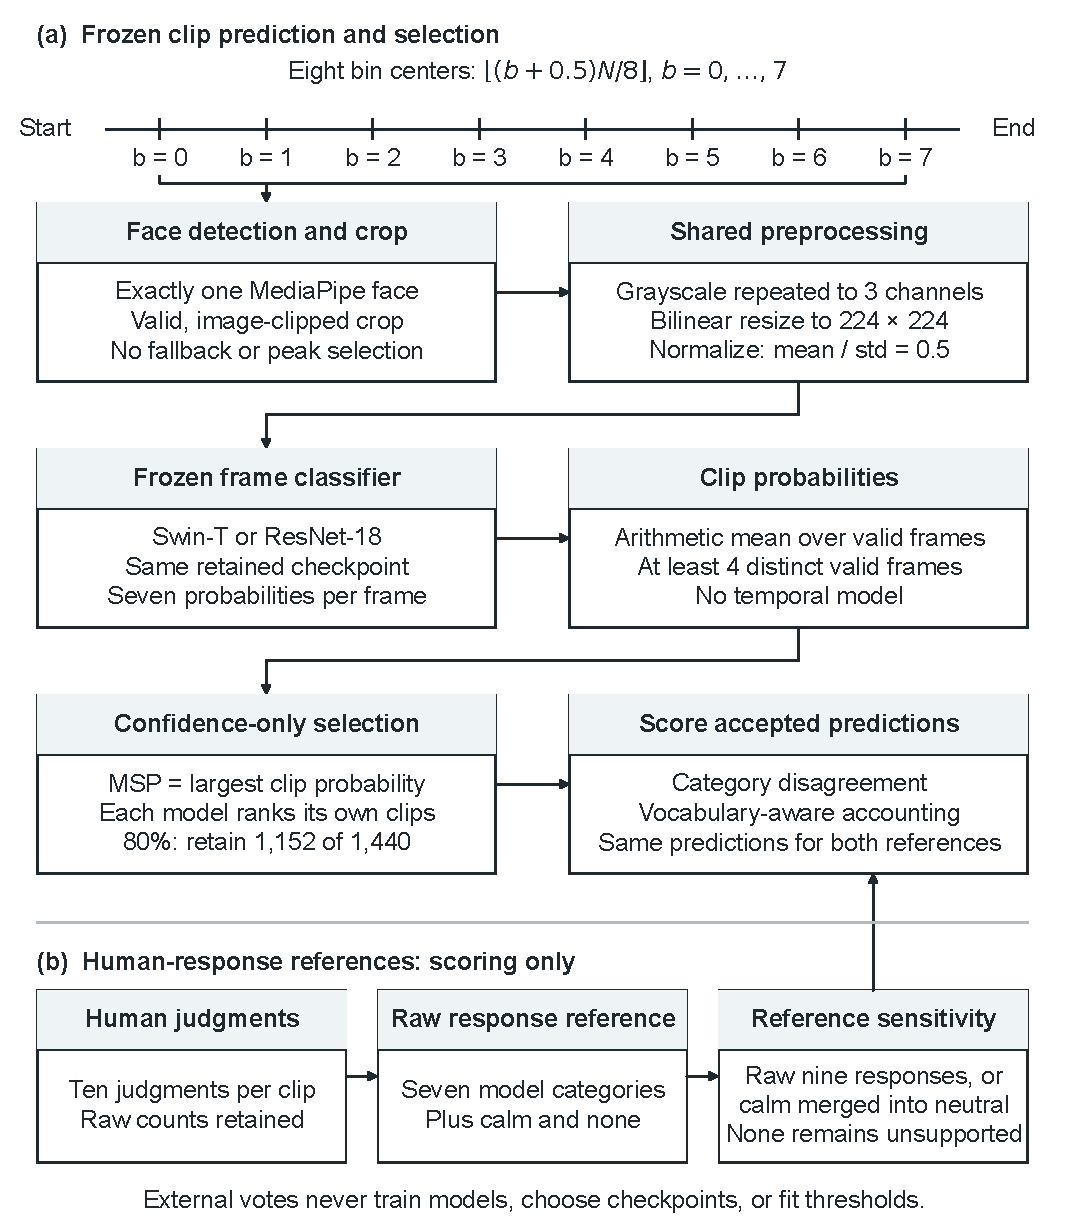
\includegraphics[width=\linewidth]{final_revision_2026_10_20/source/figures/ExternalPipeline.pdf}
\caption{Original frozen-model clip evaluation. Eight bin-center frames undergo fixed detection, cropping, preprocessing and inference. Valid-frame probabilities are averaged before clip prediction and confidence ranking. Every clip remains in the coverage denominator; votes enter scoring only. Raw and calm/neutral-merged references score unchanged outputs. Central-window aggregation is examined separately as a post hoc sensitivity}\label{fig:externalpipeline}
\end{figure}

Post hoc diagnostics retain class frequencies, every temporal bin and vote-weighted matrices $C_{ab}(A)=\sum_{i\in A}q_{ia}\mathbb I(\hat c_i=b)$. Row normalization uses accepted vote mass and is undefined for zero mass. These fractional contributions are not independent participant observations. Clip-level judgments do not establish frame accuracy. Follow-up constant-category references score all clips and the same model-fixed accepted sets; central-window aggregation tests a fixed alternative to eight-frame averaging. Both are exploratory, with no frame selection using outcomes.

\subsection{Local prototype and verification scope}
The supplementary Streamlit application is a local sender composition preview using MediaPipe \cite{lugaresi2019mediapipe}, the shared preprocessing, seven-class order and Swin head. The eight-output models are research comparisons and are not deployed in this preview. It has no recipient-side transport. Opt-in and invalid/stale-cue suppression are unvalidated design safeguards; offline calibration policies are not deployed in the app. Local processing requires the Python backend to run on the sender's machine. A categorical cue can itself be sensitive. Software checks verify numerical metrics, model contracts and failure handling, not communication effectiveness. AI assistance (OpenAI Codex) supported literature checks, code, drafting and technical verification; the authors remain responsible for the work.
